\documentclass[fleqn]{beamer}
\usepackage[english]{babel}

\usepackage{amsmath,amssymb}
\usepackage{graphicx}
\usepackage{multicol}
\usepackage{hyperref}

% vertical separator macro
\newcommand{\vsep}{
  \column{0.0\textwidth}
    \begin{tikzpicture}
      \draw[very thick,black!10] (0,0) -- (0,7.3);
    \end{tikzpicture}
}

\newcommand{\quotes}[1]{``#1''}

\newcommand{\drawkey}[1]{%
  \begingroup\normalfont
  \includegraphics[scale=.3]{keys/#1.png}%
  \endgroup
}

% More space between lines in align
\setlength{\mathindent}{0pt}
% double spacing in paragraphs
\setlength{\parskip}{1em}

% Beamer theme
\usetheme{ZMBZFMK}
\usefonttheme[onlysmall]{structurebold}
\mode<presentation>
%\setbeamercovered{transparent=10}

% align spacing
\setlength{\jot}{0pt}

% Uncomment if you wish to use a TOC

% \AtBeginSection[]
% {
%   \begin{frame}
%     \frametitle{Table of Contents}
%     \tableofcontents[currentsection]
%   \end{frame}
% }
% \AtBeginSubsection[]
% {
%   \begin{frame}
%     \frametitle{Table of Contents}
%     \tableofcontents[currentsubsection]
%   \end{frame}
% }


% Only the first Slide
\title{How to Install Intel Questa}
\author{Rich Baird}
\institute[University of Utah]{}
\date{\today}


% Title
\begin{document}
\begin{frame}
  \titlepage
\end{frame}

% Frame 1
\section{Questa Installation Guide}
\begin{frame}
  \frametitle{Motivation}
    Starting with Intel® Quartus® Prime version 21.3, the ModelSim*-Intel® FPGA edition software has been discontinued and replaced by the Questa*-Intel® FPGA. This change has since made its way to the lite edition in 21.1. \par
    Overall this is a welcome update as Modelsim has not been in active development for some time. However, the installation and licensing process can be a bit of a challenge. This guide will take you through the process of installing and setting up Questa so that you may begin writing and running your simulations.
\end{frame}

\subsection{Obtaining the software}
\begin{frame}{Software Installation}
    To begin, navigate in your preferred browser to \url{https://fpgasoftware.intel.com}. Once there, make sure that you have selected the Lite edition, and the latest release. At the time of writing, this is version 21.1.
    
\begin{figure}
    \centering
    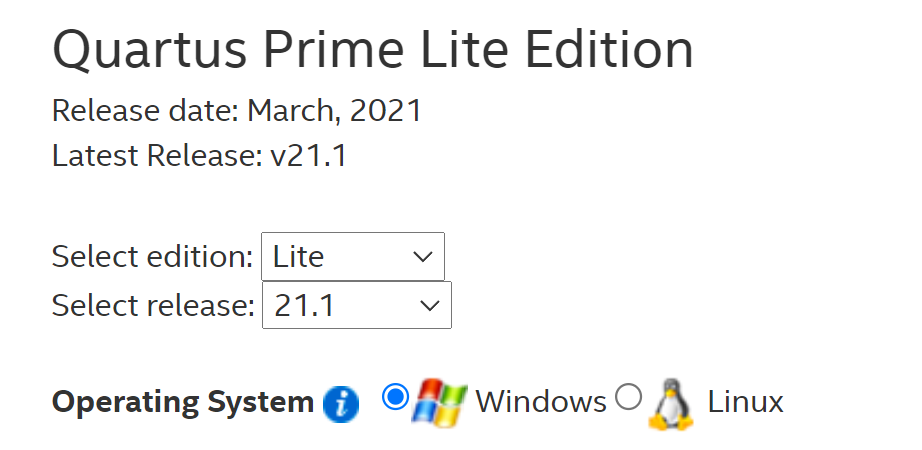
\includegraphics[scale=.5]{figures/QLite21.png}
    \caption{Ensure the correct edition and release}
    \label{fig:editionrelease}
\end{figure}
\end{frame}

\begin{frame}{Software Installation}
    Further down on the page find the download link for \quotes{Questa - Intel FPGA Edition(includes Starter Edition)}
    \begin{figure}
        \centering
        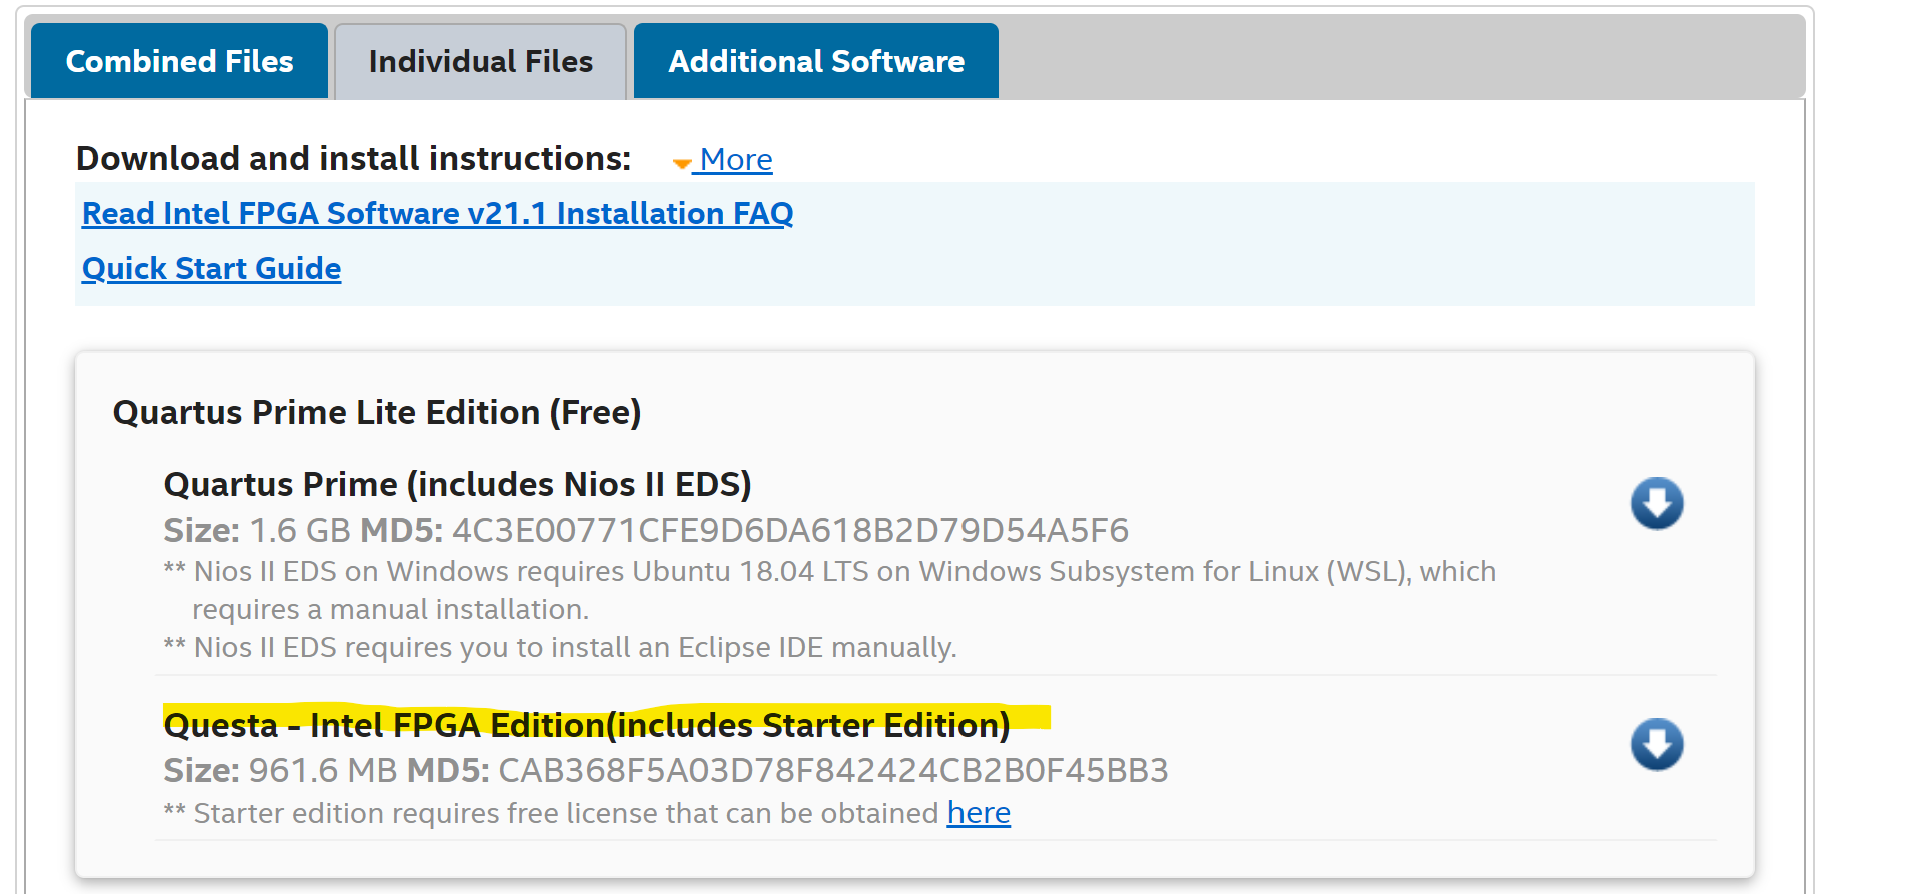
\includegraphics[scale=.4]{figures/questadl.png}
        \caption{Download Questa with the blue download arrow}
        \label{fig:my_label}
    \end{figure}
\end{frame}
\subsection{Obtaining a license}
\begin{frame}{Get a license}
    To use the software you will need a free license. This can be obtained by navigating in your preferred browser to \url{https://licensing.intel.com/}. You will be greeted with a login screen. Use your intel credentials to log in here.\par
If you are not able to log in with those credentials, you may need to register a specific account for the licensing center. Some users have reported after creating an account that they have had to wait up to 30 minutes before the licensing page would let them in. If the page redirects you to the Intel homepage, just continue trying every five minutes or so.
\end{frame}
\begin{frame}{Get a license}
    Once you have completed the registration and are able to log into the licensing site, from the menu select \quotes{Sign up for Evaluation or Free Licenses}. From that page, select the 2nd option in the table \quotes{Questa*-Intel® FPGA Starter Edition} and set the \# of seats to 1.
    \begin{multicols}{2}
        \begin{figure}
            \centering
            
\includegraphics[scale=.3]{figures/freelicenses.png}
            \caption{Sign up for Free Licenses}
            \label{fig:my_label}
        \end{figure}
        \begin{figure}
            \centering
            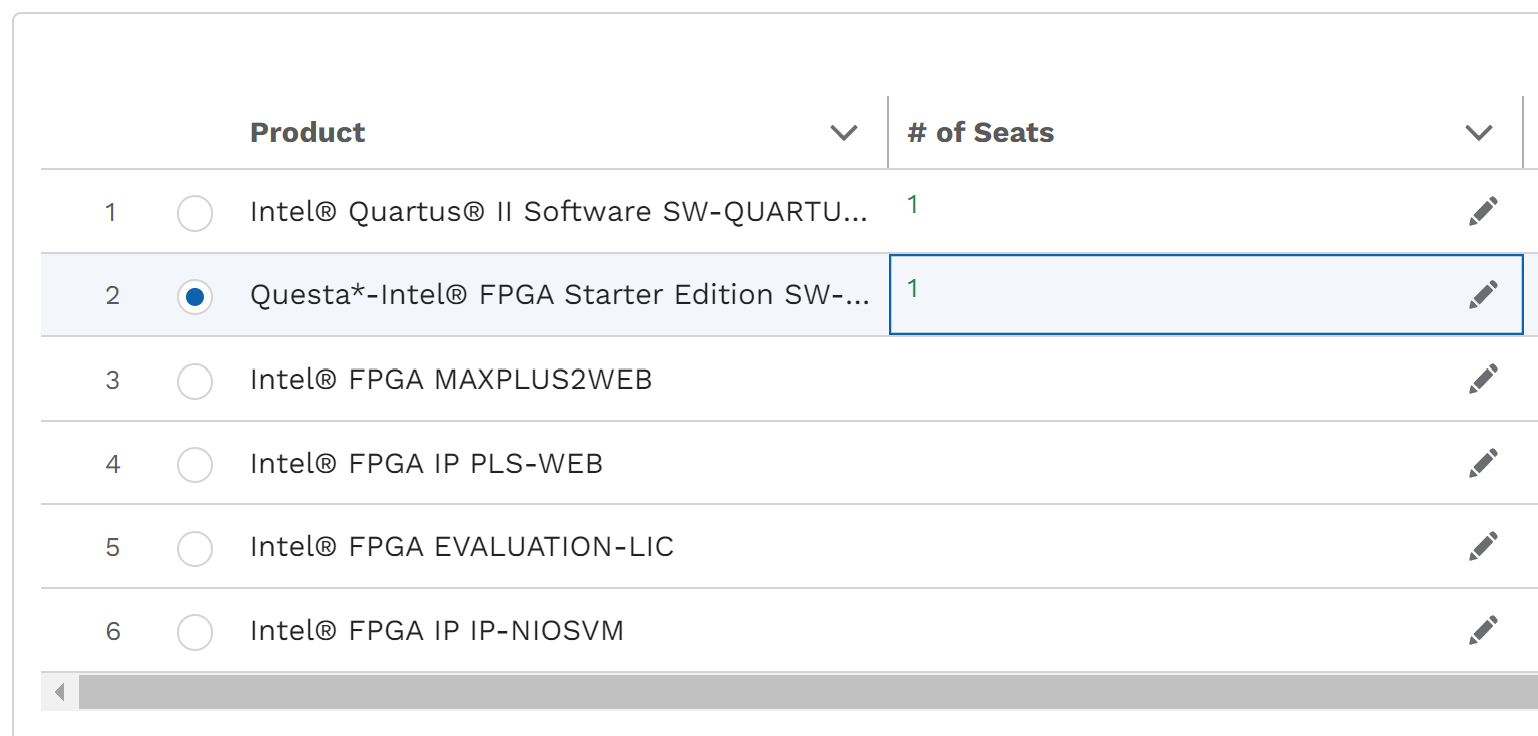
\includegraphics[scale=.3,trim={0 3cm 3cm 0},clip]{figures/questalicense.png}
            \caption{Questa License with 1 seat}
            \label{fig:my_label}
        \end{figure}
    \end{multicols}
    \vspace{-.5cm}
    Finally, mark the 2 option boxes at the bottom of the screen and press the blue \quotes{Get a License} button.
\end{frame}
\begin{frame}{Create a computer}
    In the new screen that appears, select the \quotes{+New Computer} option. Here you will need the following information \begin{itemize}
        \item Computer Name
        \item Physical NIC Address
    \end{itemize}
To obtain the first, from the launch bar of your PC, search for \quotes{This PC}. On the right side of the menu, select properties.
\vspace{-1cm}
\begin{figure}
    \centering
    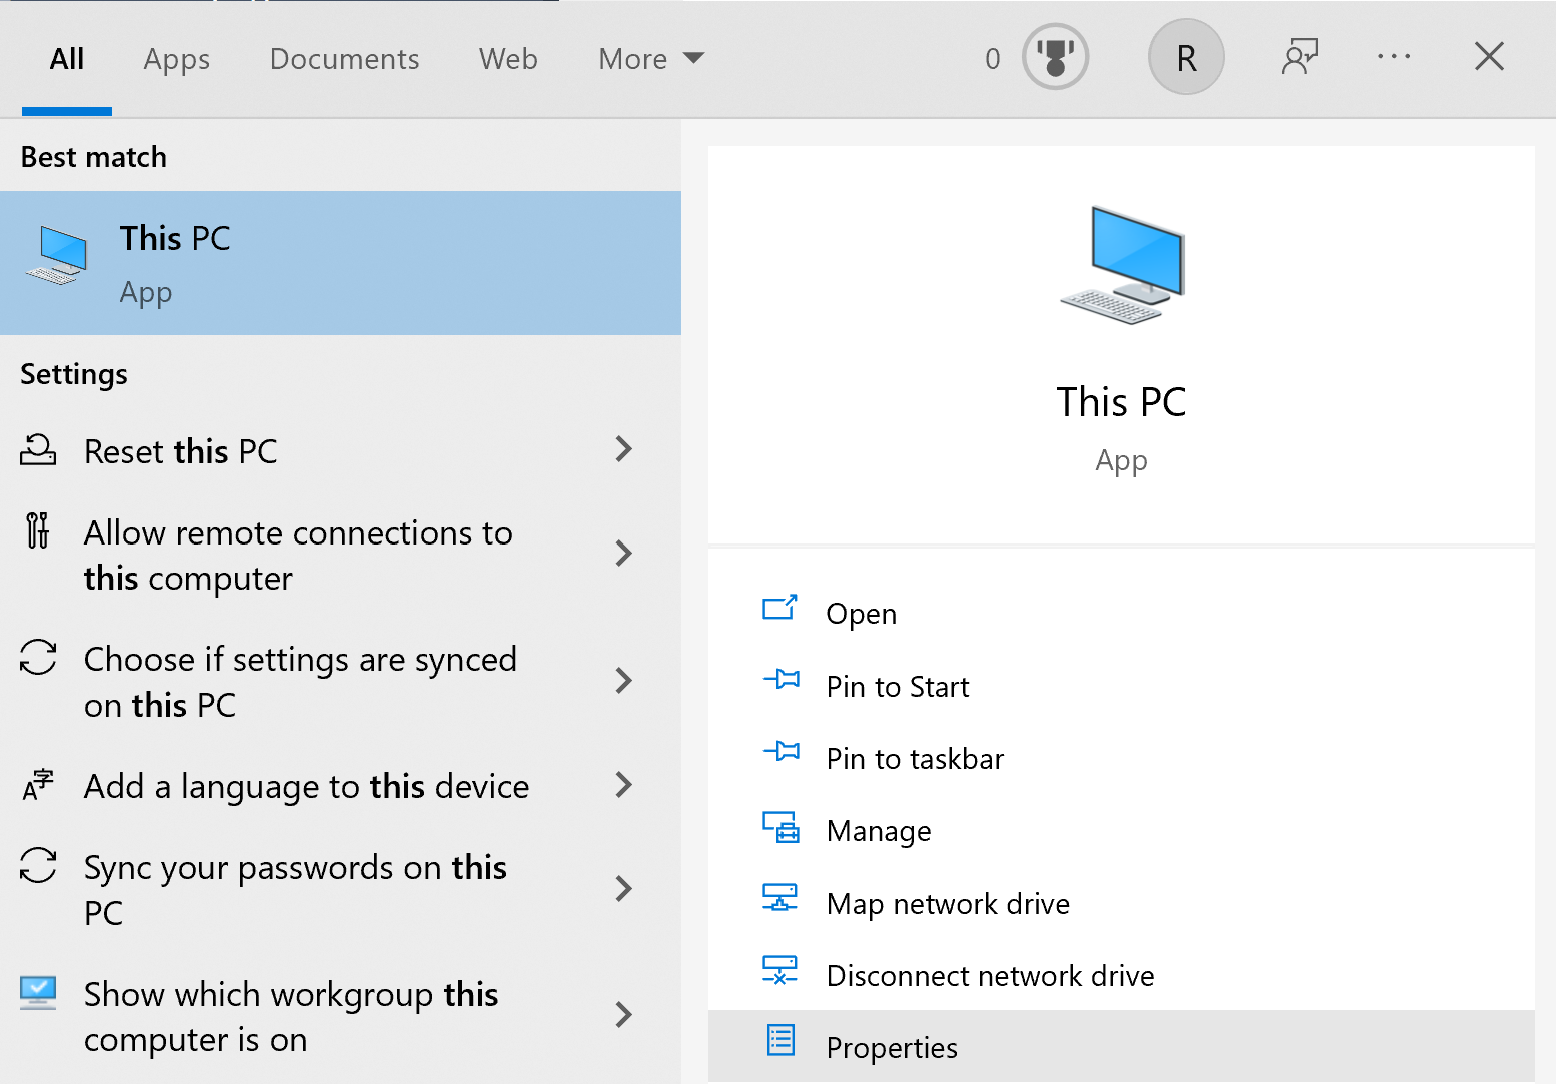
\includegraphics[scale=.2]{figures/pcproperties.png}
    \caption{Select Properties from the \quotes{This PC} menu}
    \label{fig:my_label}
\end{figure}
\end{frame}
\begin{frame}{Create a computer}
    In the properties dialog, you will find the device name under Device Specifications. Place this value in the \quotes{Computer Name} field of the Create Computer dialog on the licensing page.
    \begin{multicols}{2}
        \begin{figure}
            \centering
            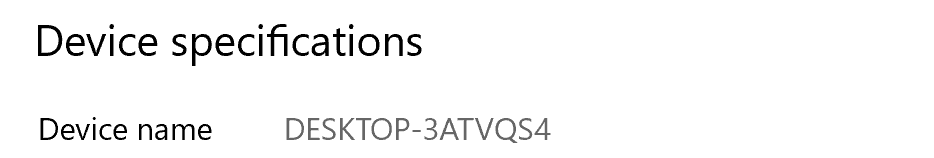
\includegraphics[scale=.4]{figures/devicename.png}
            \caption{Device name from computer properties}
            \label{fig:my_label}
        \end{figure}
        \begin{figure}
            \centering
            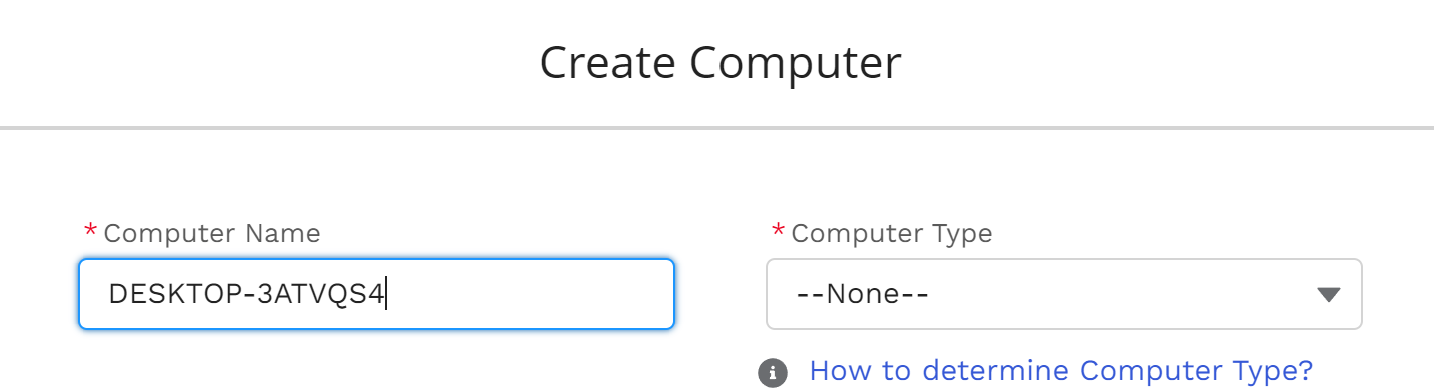
\includegraphics[scale=.3]{figures/ccmenucpuname.png}
            \caption{Create Computer Dialog}
            \label{fig:my_label}
        \end{figure}
    \end{multicols}
    Leave the properties dialog open. We will need it again later.
\end{frame}
\begin{frame}{Create a Computer}
    To obtain the physical NIC address, press \drawkey{win} + \drawkey{R} to open the run prompt. Inside the prompt type \quotes{cmd} without quotes and press OK to open the command prompt. In the command prompt that follows, type \quotes{ipconfig /all} and press enter.
    \begin{multicols}{2}
        \begin{figure}
            \centering
            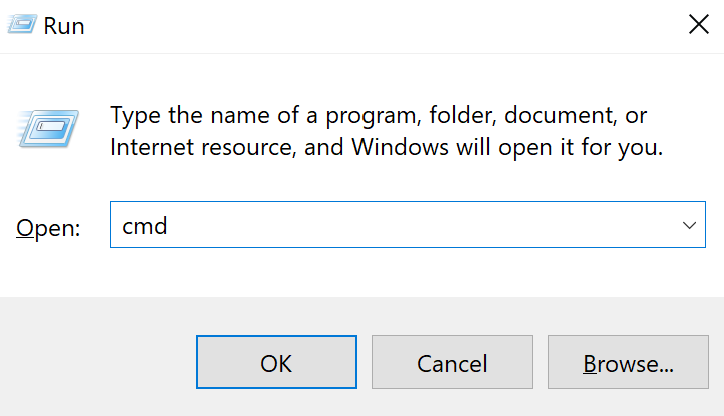
\includegraphics[scale=.5]{figures/runcmd.png}
            \caption{Run Prompt}
            \label{fig:my_label}
        \end{figure}
        \begin{figure}
            \centering
            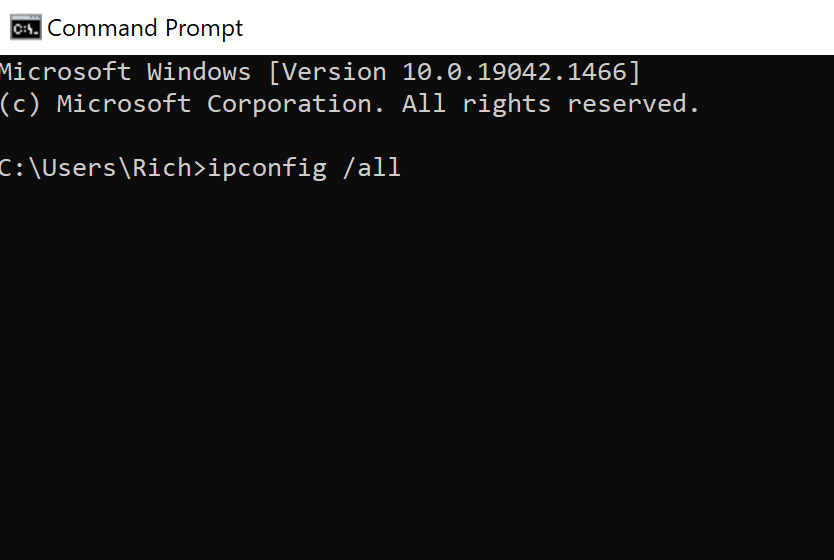
\includegraphics[scale=.5]{figures/cmd.png}
            \caption{Command prompt}
            \label{fig:my_label}
        \end{figure}
    \end{multicols}
\end{frame}
\begin{frame}{Create a Computer}
    This command will list several characteristics of your network interfaces. From this list, find the \quotes{physical address} line. Type the corresponding number without hyphens (\quotes{-}) into the Primary Computer ID field of the Create a Computer dialog. If you have multiple NICs, the dialog provides options for secondary and tertiary IDs that you can place them in. Please be aware that if you are using a virtual machine, you will need to make sure that your setup does not reinitialize mac addresses at every boot. The details of this setup are beyond the scope of this guide.
    \begin{multicols*}{2}
        \begin{figure}
            \centering
            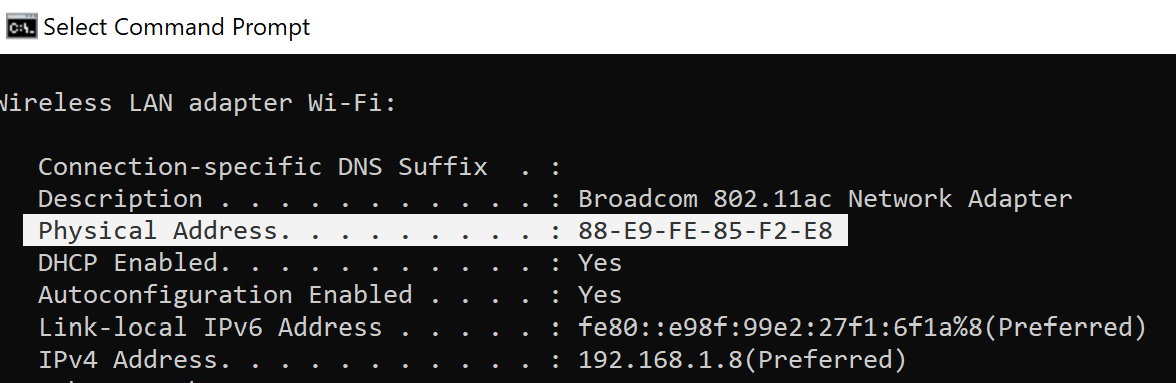
\includegraphics[scale=.3]{figures/ipconfigall.png}
            \caption{Caption}
            \label{fig:my_label}
        \end{figure}
        \begin{figure}[hbtp]
            \vspace{-1cm}
            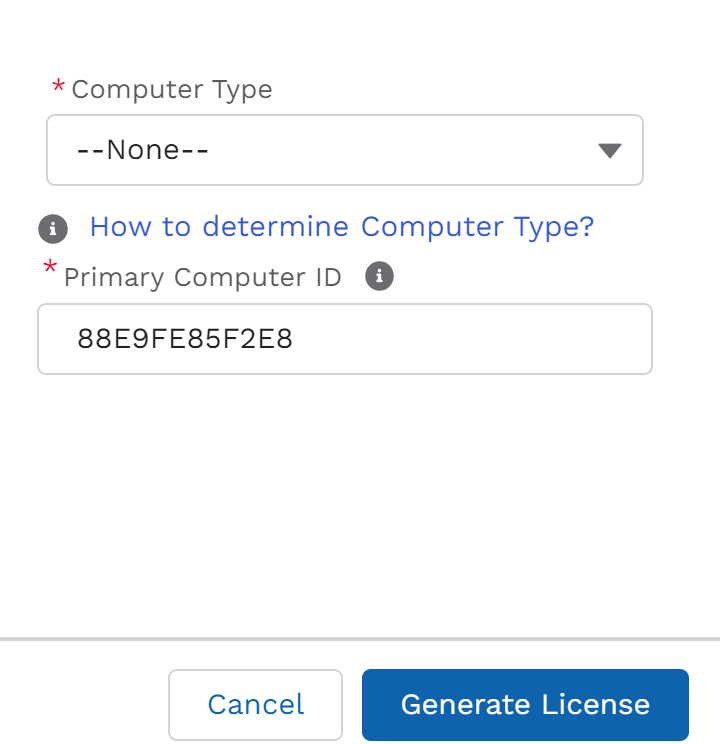
\includegraphics[scale=.6,trim={0 4cm 0 0},clip]{figures/pcid.png}
            \caption{Primary Computer ID should be the physical address}
            \label{fig:my_label}
        \end{figure}
    \end{multicols*}
\end{frame}
\begin{frame}{Create a Computer}
    Finally in the Create a Computer dialog select \quotes{License Type} and set it to fixed, and select \quotes{Primary ID} and set it to NIC. Then click on the blue \quotes{Generate License} button.
\end{frame}
\subsection{Complete Installation}
\begin{frame}{Software Installation}
    If you have already installed Quartus with Questa you can skip this step.
    \hline
    With the generated license, you are ready to install the Questa program you downloaded earlier. Be sure to select Intel FPGA \textbf{Starter} Edition, \textbf{NOT} FPGA Edition. Follow the defaults for the rest of the install.
    \begin{figure}
        \centering
        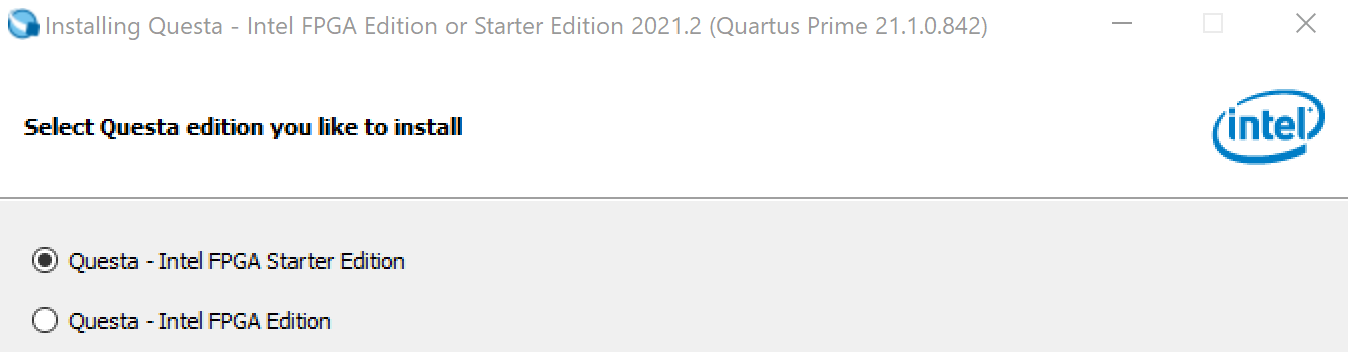
\includegraphics[scale=.5]{figures/questaintelfpgaedt.png}
        \caption{Select Intel FPGA Edition}
        \label{fig:my_label}
    \end{figure}
\end{frame}
\subsection{Installing the license}
\begin{frame}{License Installation}
    Once the software is installed, download the .dat license file sent to the email associated with your login and save it to a location where it won't get accidentally deleted.
    \begin{figure}
        \centering
        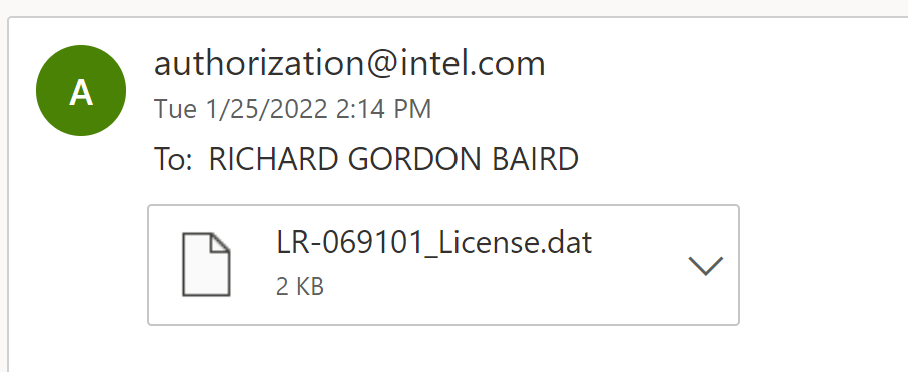
\includegraphics[scale=.8]{figures/licensedat.png}
        \caption{Save the .dat file to a safe location}
        \label{fig:my_label}
    \end{figure}
\end{frame}
\begin{frame}{License Installation}
   Once saved go back to the computer properties dialog from slide 7. On the right side -- or bottom if the dialog isn't expanded -- find and select \quotes{advanced System Settings}.
   \begin{figure}
       \centering
       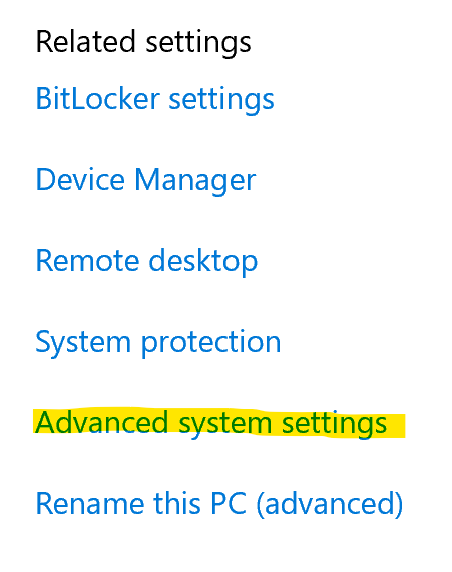
\includegraphics[scale=.5]{figures/advancedsettings.png}
       \caption{Advanced System Settings}
       \label{fig:my_label}
   \end{figure}
\end{frame}
\begin{frame}{License Installation}
    From here Select \quotes{Environment Variables} $\longrightarrow$ \quotes{User Variables} $\longrightarrow$ \quotes{New}\par
    From here add the variable name \quotes{LM\_LICENSE\_FILE}. Set as the value the path to the .dat file downloaded earlier. Press Okay and Okay and close the system properties. See the next slide for a visual guide.
\end{frame}
\begin{frame}{License Installation}
    \begin{figure}
        \centering
        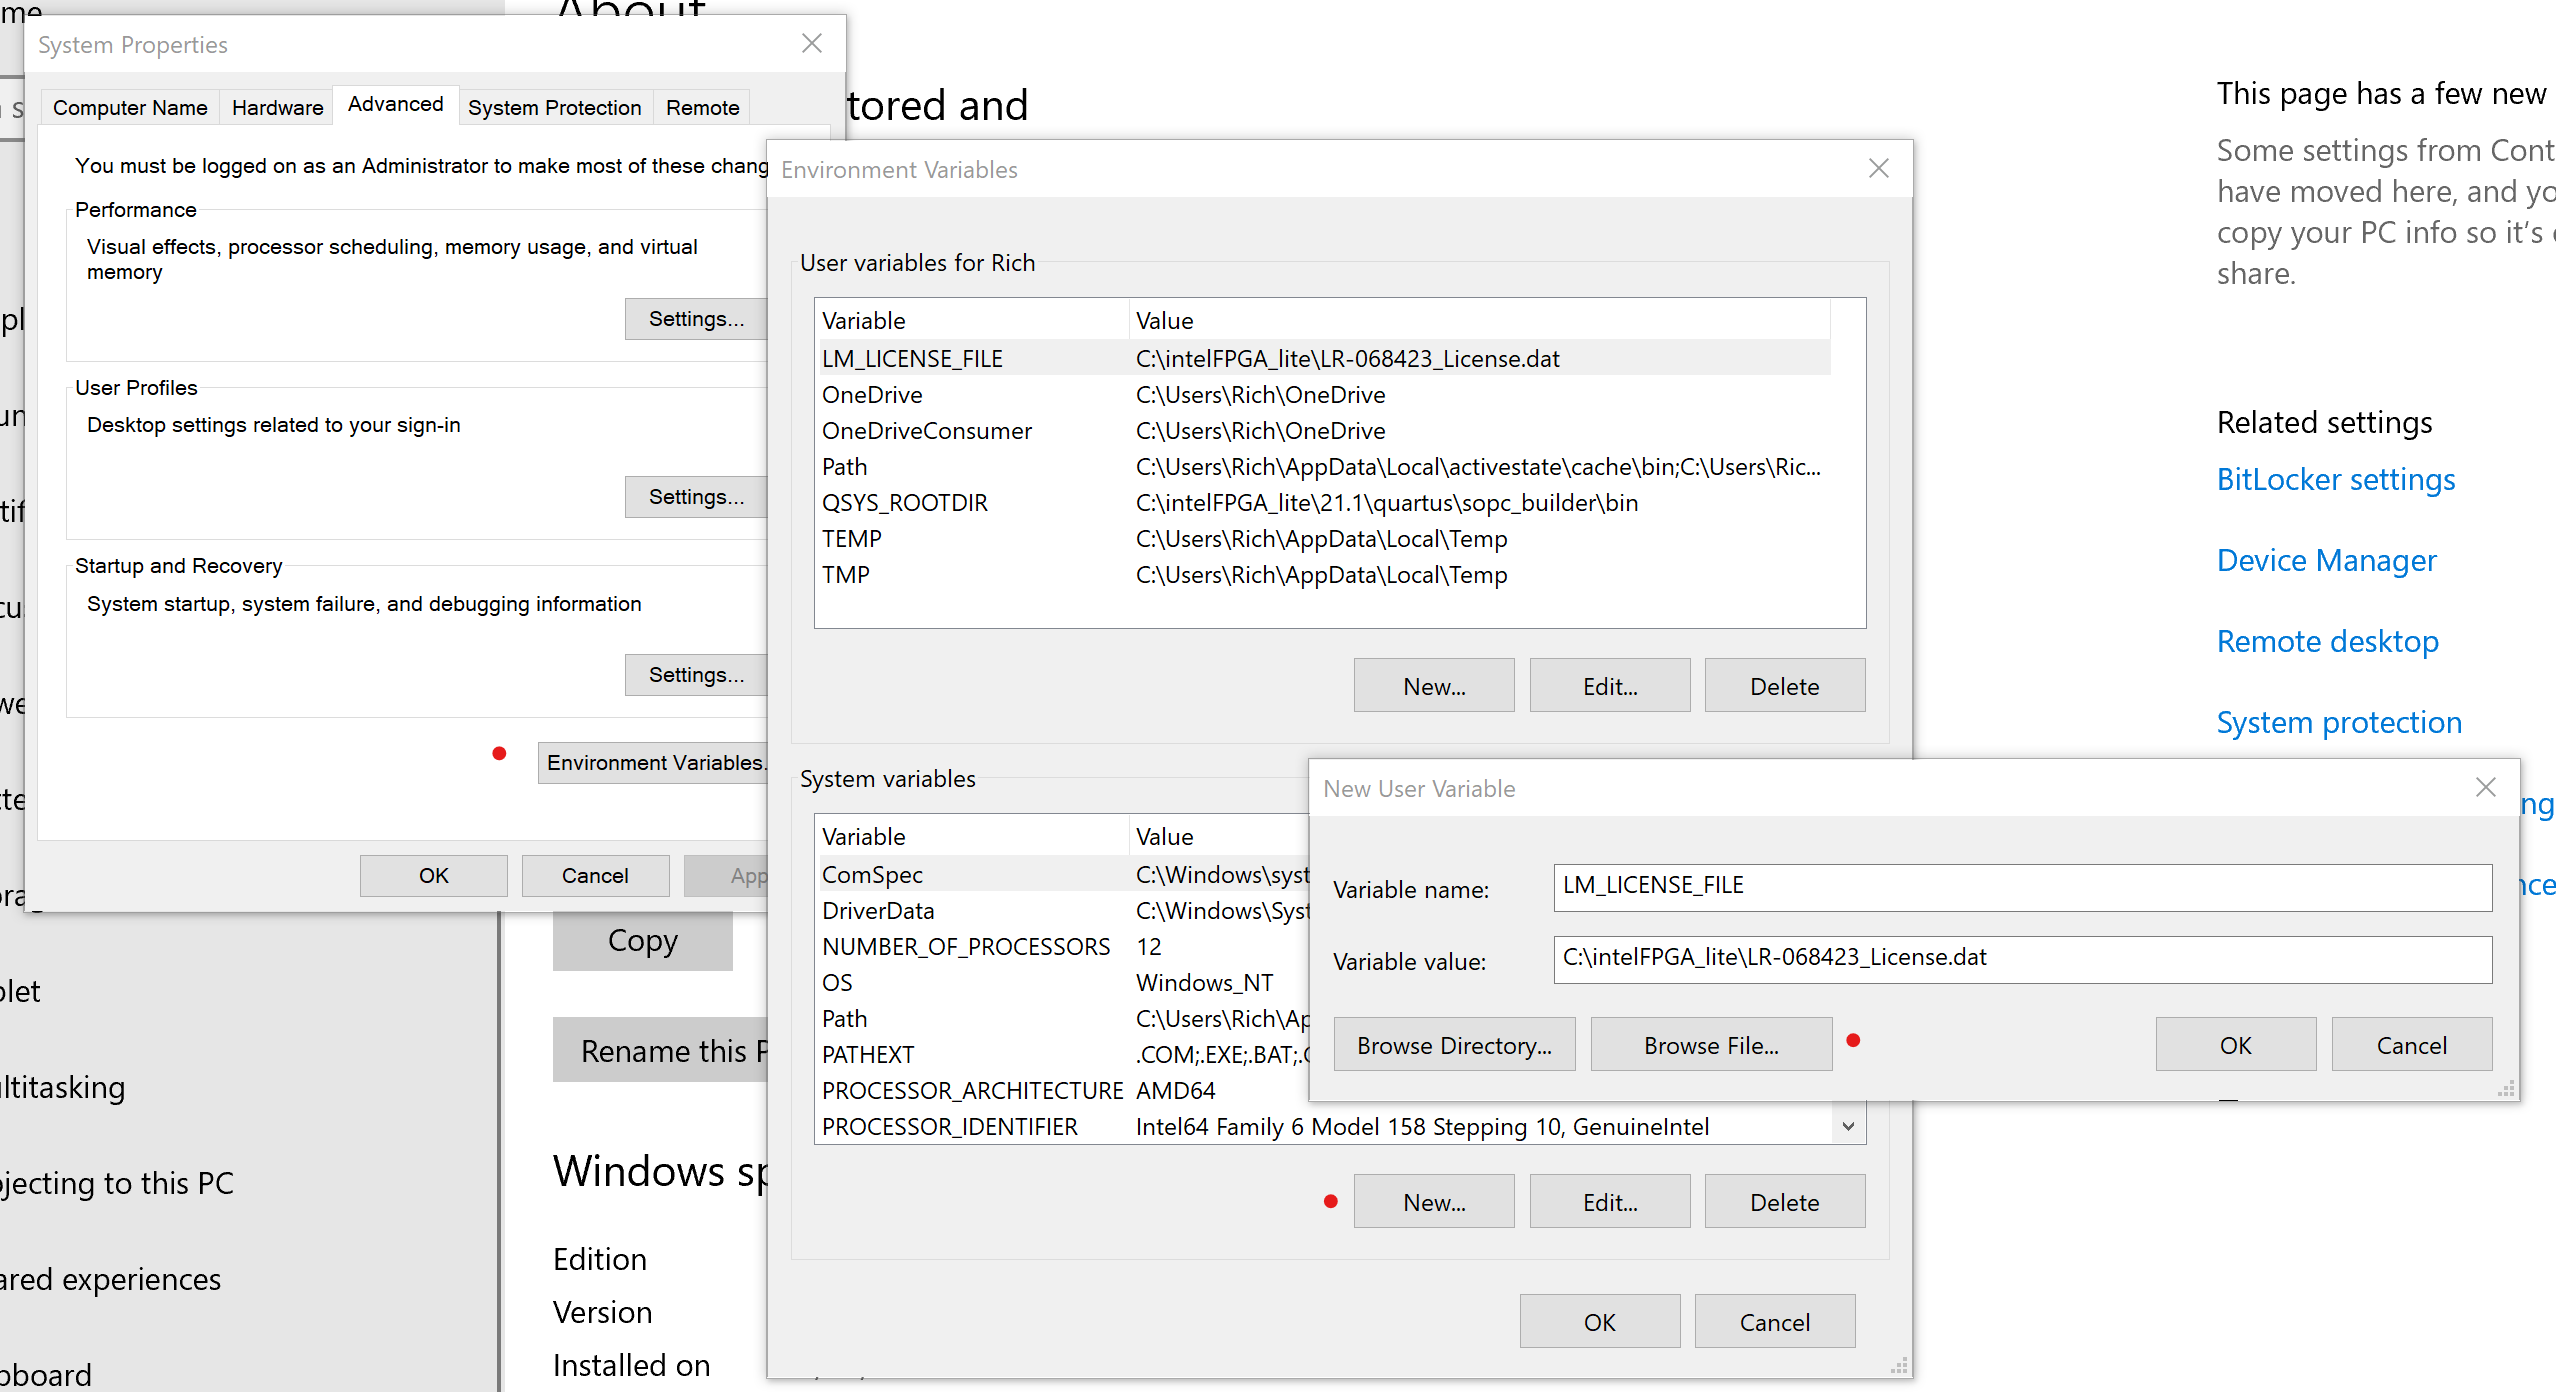
\includegraphics[height=16em]{figures/envvars.png}
        \caption{Add environment variable}
        \label{fig:my_label}
    \end{figure}
\end{frame}
\subsection{Connect Questa and Quartus}
\begin{frame}{Quartus Setup}
    Launch Quartus and go to tools $\longrightarrow$ options $\longrightarrow$ EDA Tool Options $\longrightarrow$ Questa Intel FPGA\par
    Type the location of the Questa executable in the space provided. On windows the default location is C:\textbackslash{}intelFPGA\textbackslash{}21.1\textbackslash{}questa\_fse\textbackslash{}win64
    \begin{multicols}{2}
        \begin{figure}
        \centering
        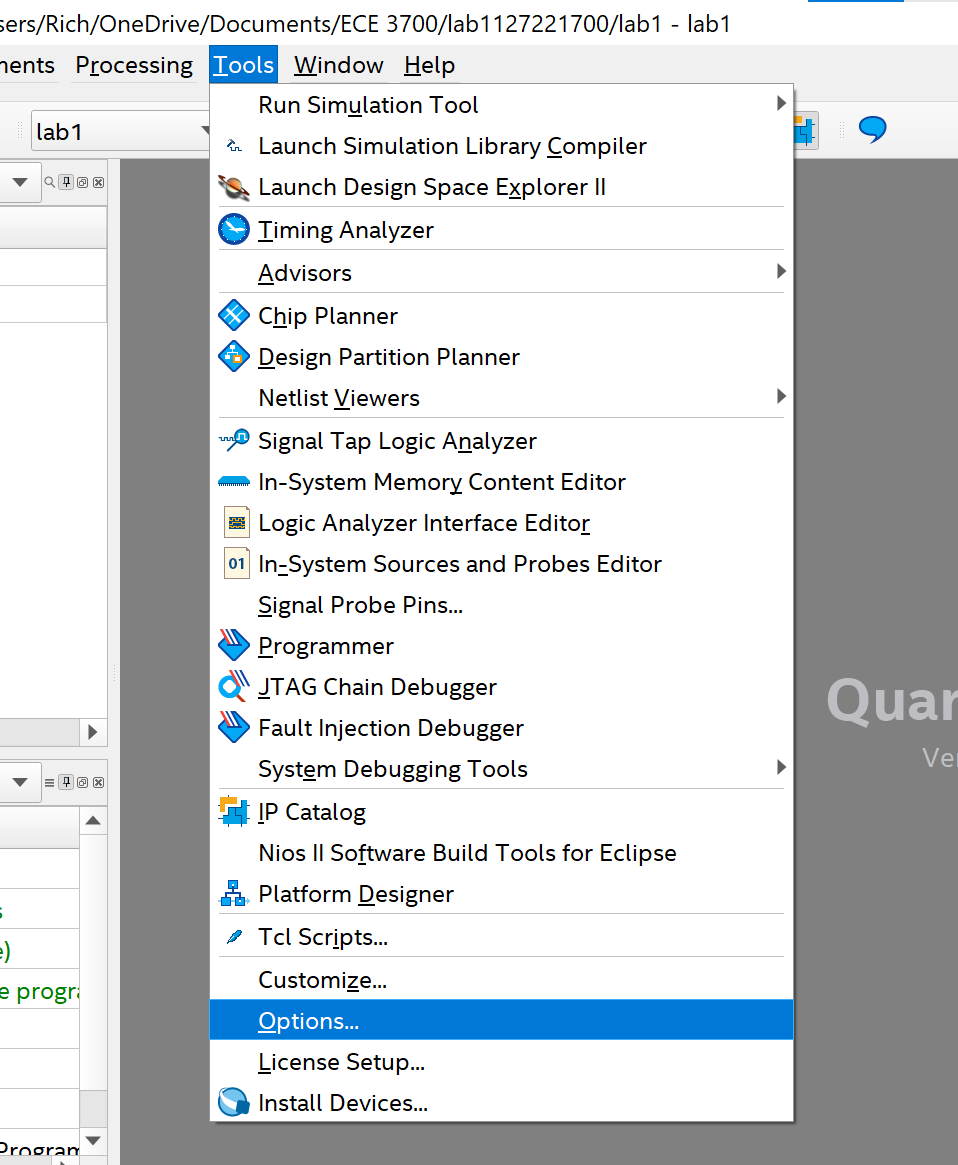
\includegraphics[scale=.3]{figures/quartusopts.png}
        \label{fig:my_label}
    \end{figure}
    \begin{figure}
        \centering
        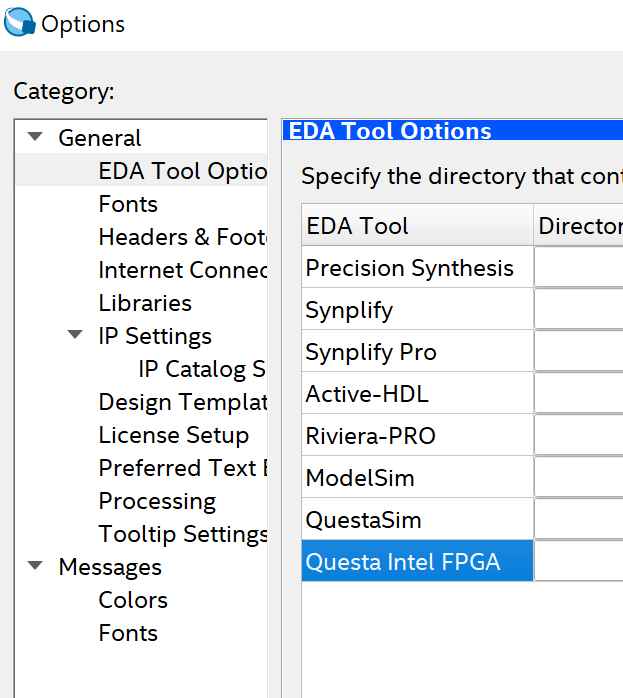
\includegraphics[scale=.5]{figures/edatool.png}
        \label{fig:my_label}
    \end{figure}
    \end{multicols}
\end{frame}
\begin{frame}{Quartus Setup}
    Go to Assignments $\longrightarrow$ Settings $\longrightarrow$ EDA Tool Settings $\longrightarrow$ Simulation\par
    Select the \quotes{Tool name:} drop down and choose \quotes{Questa Intel FPGA} and press okay.
    \begin{figure}
        \centering
        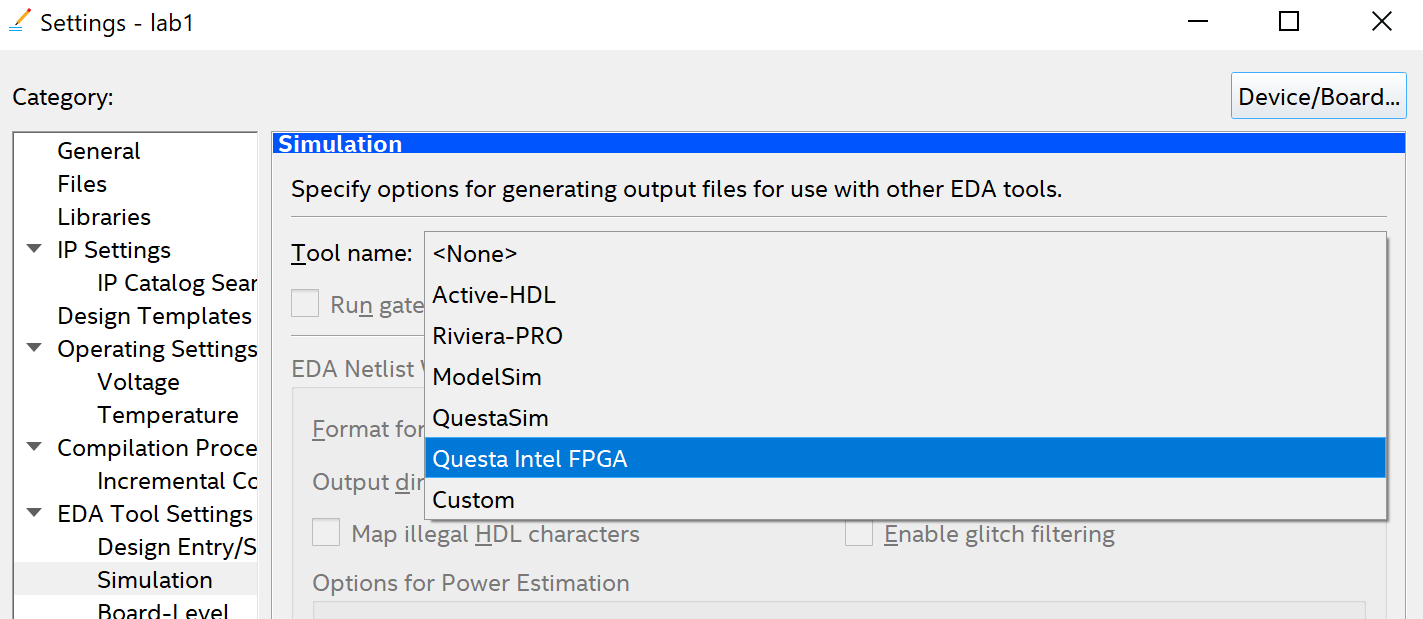
\includegraphics[scale=.5]{figures/simtool.png}
        \label{fig:my_label}
    \end{figure}
\end{frame}
\end{document}